\section{Reinigungsanlagen - Wässrige Teilreinigung}
\label{ch_03Wässrige Teilreinigung}
\begin{itemize}
	\item Funktionsweise und Besonderheiten von wasserbasierten Teilreinigungsanlagen
\end{itemize}

\begin{figure}[h]
	\centering
	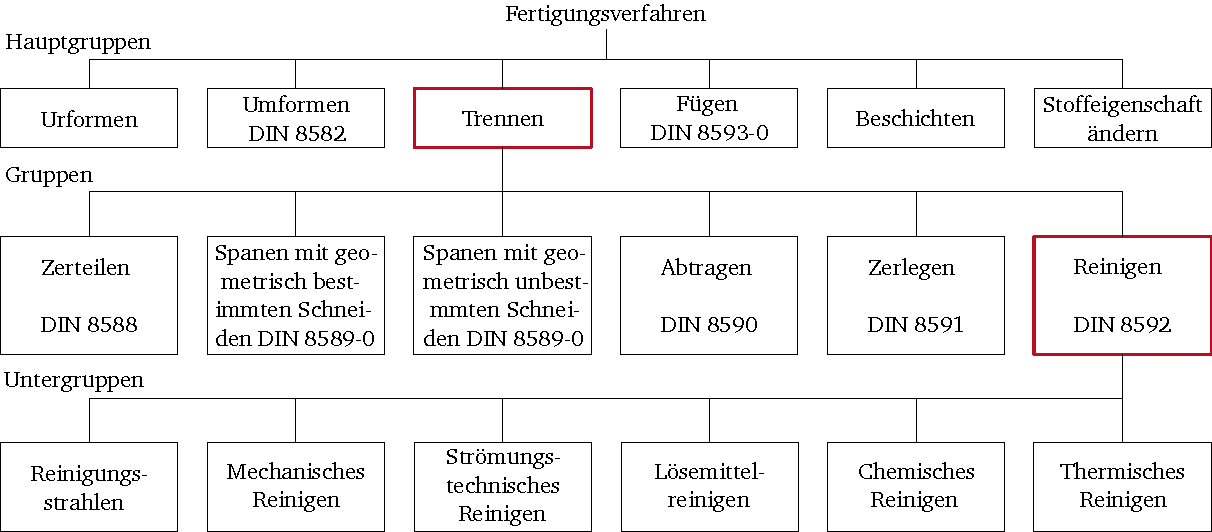
\includegraphics[width=400pt]{figures/03_Grundlagen/Hauptgruppen der Fertigungsverfahren - Reinigen.pdf}
	\caption{Hauptgruppen der Fertigungsverfahren - Reinigen, nach \cite{DIN8580}}
	\label{fig_03Hauptgruppen der Fertigungsverfahren - Reinigen}
\end{figure}

Die Abbildung \ref{fig_03Hauptgruppen der Fertigungsverfahren - Reinigen} zeigt die Einteilung der Reinigungsverfahren in die verschiedenen Hauptgruppen der Fertigungsverfahren. Die Einteilung erfolgt in sechs Hauptgruppen: Urformen, Umformen, Trennen, Fügen, Beschichten und Stoffeigenschaft ändern. Innerhalb dieser Hauptgruppen können alle existierenden und denkbaren Fertigungsverfahren eingeordnet werden.\\

In der Abbildung \ref{fig_03Hauptgruppen der Fertigungsverfahren - Reinigen} wird deutlich, dass die Reinigungsverfahren der Hauptgruppe \glqq Trennen\grqq~ zugeordnet sind, welche weiter in die Gruppe \glqq Reinigen\grqq~ (DIN 8592) unterteilt wird \cite{dindeutschesinstitutfurnormunge.v.FertigungsverfahrenReinigenEinordnungBeuthVerlagGmbH}. Diese Gruppe umfasst mehrere Untergruppen, die spezifische Reinigungsverfahren darstellen, wie mechanisches Reinigen, strömungstechnisches Reinigen, Lösemittelreinigen, chemisches Reinigen und thermisches Reinigen.\\

Das Entfernen unerwünschter Substanzen (Verunreinigungen) von Werkstückoberflächen erfolgt bis zu einem festgelegten, vereinbarten oder möglichen Reinheitsgrad. Der erreichbare Reinheitsgrad hängt dabei sowohl vom angewandten Reinigungsverfahren als auch von der Art und Beschaffenheit der Verunreinigungen ab \cite{dindeutschesinstitutfurnormunge.v.FertigungsverfahrenReinigenEinordnungBeuthVerlagGmbH}. Eine solche Reinigung kann beispielsweise das Entfetten, Dekontaminieren oder Entfernen von Beschichtungen umfassen, wie in \cite{dindeutschesinstitutfurnormunge.v.FertigungsverfahrenReinigenEinordnungBeuthVerlagGmbH} beschrieben.\\

Das Strömungstechnische Reinigen ist ein spezielles Verfahren innerhalb der Gruppe \grqq Reinigen\glqq~. Es beschreibt den Prozess, bei dem lose anhaftende Verunreinigungen durch strömende Gase oder Flüssigkeiten entfernt werden \cite{dindeutschesinstitutfurnormunge.v.FertigungsverfahrenReinigenEinordnungBeuthVerlagGmbH}. Dies umfasst Verfahren wie Waschen und Spülen, Abblasen, Absaugen sowie Ultraschallreinigung. In industriellen Anwendungen werden häufig verschiedene Reinigungsverfahren miteinander kombiniert, um den hohen Anforderungen an die Reinigungsleistung gerecht zu werden. Dies trifft auch auf wässrige Teilereinigungsmaschinen (APCMs) zu, weshalb sie nicht ausschließlich einem der definierten Reinigungsverfahren zugeordnet werden können \cite{jungeBeitragZurEnergieeffizienzbewertung2019}. Diese Kombinationen ermöglichen die Entwicklung von Reinigungsanlagen, die in der Lage sind, komplexe Systeme abzubilden und durch einen hohen Grad an Automatisierung nahezu autonom zu arbeiten \cite{jungeBeitragZurEnergieeffizienzbewertung2019}. Die Komplexität des Reinigungsprozesses hängt vor allem von der Automatisierungsstufe und der Anzahl der integrierten Prozessphasen ab. Zusätzlich spielt die Handhabung der Reinigungsgüter eine wesentliche Rolle bei der Bestimmung der Gesamtkomplexität \cite{wullsteinAuswahlUndOptimale2004}.\\

Marktanalysen haben ergeben, dass die wässrige Reinigung die am häufigsten angewendete Methode in der industriellen Reinigung ist und ihr Anteil stetig wächst. Im Jahr 2007 nutzten 59 \% der befragten Unternehmen wässrige Reinigungsverfahren; dieser Anteil stieg bis 2012 auf 84 \% und erreichte 2020 einen Wert von 86 \% {Bilz13, S. 21; Rögn21a, S. 45}. Parallel dazu erhöhte sich der Umsatzanteil der wässrigen Reinigung bei Herstellern von Reinigungsmaschinen von 58 \% im Jahr 2007 auf 68 \% im Jahr 2012 und weiter auf 84 \% im Jahr 2020 {Bilz13, S. 21; Rögn21a, S. 45}. Diese Daten unterstreichen die zunehmende Bedeutung wasserbasierter Teilereinigungsmaschinen in der Industrie. Dies erhöht das Potenzial und die Skalierbarkeit der in dieser Arbeit untersuchten Maßnahmen zur Energieflexibilisierung erheblich. (Quellen Fraunhofer - noch keine Zugang gefunden)\\


In dieser Arbeit wird eine wässrige Teilereinigungsmaschine energetisch flexibel betrieben. Daher ist es zunächst notwendig, den Begriff der wässrigen Teilereinigungsmaschine zu definieren. Derzeit existiert keine einheitliche Definition. \textcite{fuhrlander-volkerModellingControlAqueous2023} hat in seiner Arbeit versucht, eine solche Definition zu geben. Er beschreibt die wässrige Teilereinigungsmaschine als eine Produktionsmaschine, die fluidische Reinigung mit chemischer und Lösemittelreinigung kombiniert, um industrielle Teile mit wässrigen Reinigungsflüssigkeiten zu säubern \cite{fuhrlander-volkerModellingControlAqueous2023, dindeutschesinstitutfurnormunge.v.FertigungsverfahrenReinigenEinordnungBeuthVerlagGmbH, OekologischeUndOekonomische}.\\

Automatisierte Anlagen für nass-chemische Reinigungsprozesse lassen sich nach der Anzahl und Ausstattung der Prozesskammern klassifizieren, in denen die Bauteile gereinigt werden \cite{OekologischeUndOekonomische}. Die Konstruktion dieser Anlagen wird durch Faktoren wie Verschmutzungsgrad, Art des Reinigungsobjekts und angestrebte Zielsauberkeit bestimmt. Alle Reinigungsanlagen zeichnen sich durch grundlegende Komponenten aus, zu denen der Reinigungsbereich in Form einer Kammer oder eines Beckens, die Medienzufuhr- und Sammelbehälter sowie Einrichtungen zur Verunreinigungsabscheidung und -extraktion gehören \cite{jungeBeitragZurEnergieeffizienzbewertung2019}. Für Anlagen, die hohe technische Sauberkeitsanforderungen erfüllen müssen, existieren grundsätzlich zwei Verfahrensalternativen, die sich hauptsächlich durch die Anzahl der Prozesskammern unterscheiden \cite{OekologischeUndOekonomische}.\\

Einkammer-Reinigungsanlagen, wie der Name bereits andeutet, bestehen aus einer einzigen Prozesskammer. Diese Kammer wird nach der Befüllung mit dem Reinigungsgut teilweise oder vollständig mit Reinigungsflüssigkeit und/oder Spülmedium gefüllt. Häufig sind diese Anlagen mit Techniken wie Ultraschall- und Umflutverfahren ausgestattet. Separate Spül- und Reinigungstanks versorgen die Prozesskammer mit den erforderlichen Medien. Das Reinigungsgut verbleibt während des gesamten Reinigungsprozesses in der Kammer, wodurch diese Anlagen besonders für den Chargenbetrieb geeignet sind.\\

Mehrkammer-Reinigungsanlagen hingegen bringen das Reinigungsgut durch mehrere Prozesskammern und können allerdings ebenfalls im Chargenbetrieb betrieben werden. Im Gegensatz zu Einkammer-APCMs sind sie in der Lage, mehrere Chargen gleichzeitig zu reinigen. Darüber hinaus existieren wasserbasierte Teilereinigungsmaschinen, die kontinuierlich arbeiten. Typischerweise sind drei bis sechs offene Prozesskammern vorhanden, die jeweils mit verschiedenen Reinigungs- oder Spülmedien befüllt sind. Diese Kammern sind in einer geschlossenen Struktur miteinander verbunden. In den einzelnen Prozesskammern wird meist Ultraschall als mechanische Reinigungskomponente eingesetzt. Anders als bei Einkammer-Reinigungsanlagen steht bei Mehrkammer-Reinigungsanlagen nicht das Umfluten im Vordergrund, sondern eine Umwälzung des Mediums mit einem geringen Volumenstrom, um die Medien durch Filtration und Ölabscheidung aufzubereiten. Das Reinigungsgut wird von einer Kammer zur nächsten bewegt, wodurch die Restverschmutzung bei jedem Schritt reduziert wird. Dank der kontinuierlichen Aufbereitung der Reinigungs- und Spülmedien können diese Anlagen als Durchlauflinie betrieben werden \cite{OekologischeUndOekonomische}.\\ 

(vllt. noch Umfluten und Ultraschall erklären?)\\

Beide Anlagentypen bieten ökonomische und ökologische Vorteile im Betrieb, welche in Tabelle \ref{tab_03Vergleich der Eigenschaften der Anlagentypen} verglichen werden. Aufgrund ihrer baulichen Unterschiede unterscheiden sich auch die Prozessabläufe der Reinigung. Während die Abfolge der Reinigungsschritte in Mehrkammer-Reinigungsanlagen durch die Anordnung der Kammern festgelegt ist, erlaubt die Steuerung der Prozesse in Einkammer-Reinigungsanlagen eine höhere Flexibilität, siehe Tabelle \ref{tab_03Vergleich der Eigenschaften der Anlagentypen}. Die einzelnen Prozessschritte können je nach Betriebsgröße variiert werden, um den spezifischen Anforderungen der Reinigungsaufgabe gerecht zu werden.\\

\begin{table}[H] % die Tabelle hier
	\centering
	% Der hier eingefügte Code ist der generierte Code aus dem Tables Generator
\begin{tabular}{|l|c|c|}
	\hline
	\textbf{Eigenschaften}            & \textbf{\begin{tabular}[c]{@{}c@{}}Einkammer-\\ Anlage\end{tabular}} & \textbf{\begin{tabular}[c]{@{}c@{}}Mehrkammer-\\ Reinigungsanlage\end{tabular}} \\ \hline
	Erreichbare technische Sauberkeit & gut                                                                  & sehr gut                                                                        \\ \hline
	Flexibilität (Prozessanpassung)   & sehr gut                                                             & gut                                                                             \\ \hline
	Bauteildurchsatz                  & gering                                                               & hoch                                                                            \\ \hline
	Platzbedarf                       & gering                                                               & hoch                                                                            \\ \hline
	Investitionsausgaben              & gering                                                               & hoch                                                                            \\ \hline
\end{tabular}
	\caption{Vergleich der Eigenschaften der Anlagentypen, nach \cite{OekologischeUndOekonomische}}
	\label{tab_03Vergleich der Eigenschaften der Anlagentypen} % ein Label für Referenzen
\end{table}
 
 Der Reinigungsprozess in wasserbasierten Teilereinigungsmaschinen (APCMs) umfasst drei Hauptphasen {Durk06, S. 2--3}:
 
 \begin{enumerate}
 	\item \textbf{Reinigung:} In diesem Schritt wird der Schmutz mithilfe eines wässrigen Reinigungsmittels vom Bauteil gelöst.
 	\item \textbf{Spülen:} Hierbei wird die entstandene Emulsion aus Reinigungsmittel und Schmutz verdünnt oder verdrängt, bis alle Verunreinigungen vollständig entfernt sind.
 	\item \textbf{Trocknung:} Schließlich erfolgt die Trennung des Bauteils von der Reinigungsflüssigkeit, sodass das Bauteil trocken ist.
 \end{enumerate}
 
 Jede dieser Phasen ist entscheidend, um ein hohes Maß an Reinigungseffizienz und -qualität zu gewährleisten {Durk06, S. 3}. (schauen wie es in bei meiner DLRA ist (sieh Part Fuhrländer und schreiben was anders ist - ob spülen und Reinigen kombiniert etc.). 
 
 Der Reinigungsprozess in wasserbasierten Teilereinigungsmaschinen (APCMs) ist ein komplexes Zusammenspiel mehrerer Einflussfaktoren. Der Sinnersche Kreis ist ein etabliertes Modell, das diese Einflussfaktoren in vier Hauptkategorien einteilt: Temperatur, Chemie, Mechanik und Zeit. Diese Faktoren sind entscheidend für die Effizienz und Effektivität des Reinigungsprozesses (Sinner, Rust, Wildbrett, Junge 19).\\
 
 Nach Wildbrett wird der Sinnersche Kreis um drei zusätzliche Komponenten erweitert: Verunreinigung, Reinigungsgut und Reinigungsverfahren, siehe Abbildung \ref{fig_03Erweiterter Sinnerscher Waschkreis} Das Zusammenspiel dieser Komponenten definiert das gesamte Reinigungssystem und passt den ursprünglichen Ansatz an die spezifischen Anforderungen der industriellen Reinigung an [Angerer].\\
 
 Innerhalb der Komponente Reinigungsverfahren sind die klassischen Faktoren Temperatur, Chemie, Mechanik und Zeit eingegliedert. Diese müssen sorgfältig auf die spezifische Verunreinigung und das Reinigungsgut abgestimmt werden. Diese Faktoren beeinflussen sich gegenseitig und können durch entsprechende Anpassungen kompensiert werden. Eine präzise Abstimmung ist notwendig, um den Reinigungserfolg sicherzustellen und die Wirtschaftlichkeit des Prozesses zu maximieren [öknomisch und ökologisch], Rögn21b].\\
 
 Wenn beispielsweise die Reinigungszeit verkürzt werden soll, muss mindestens einer der anderen Faktoren, wie die Temperatur oder der Einsatz von Chemikalien, erhöht werden. Dies kann die Reinigungszeit verkürzen, jedoch sind dabei die Umwelt- und Kostenaspekte zu berücksichtigen. Gleichzeitig müssen die Materialeigenschaften des Reinigungsguts beachtet werden, da hohe Temperaturen oder intensive mechanische Einwirkungen das Material schädigen können. Um ein zufriedenstellendes Reinigungsergebnis zu erzielen, muss das Reinigungsmedium an die Art, Beschaffenheit und Menge des Schmutzes sowie an die Form und das Material des zu reinigenden Teils angepasst werden [Angerer, Junge19].\\
 
 Die beschriebenen Zusammenhänge verdeutlichen die Komplexität der Nassreinigungsverfahren und das damit verbundene Potenzial für Prozessoptimierungen. Die Auswahl geeigneter Reinigungsverfahren und die präzise Einstellung der Prozessparameter erfordert umfassendes Fachwissen über die Wechselwirkungen der Einflussgrößen. Ein wachsendes Verständnis für diese verfahrenstechnischen Zusammenhänge bei den Nutzern von Reinigungstechnologien ermöglicht die Optimierung der Prozessketten [ökonomisch und ökologisch].\\
 
 Bei der Implementierung von Maßnahmen zur Energieflexibilisierung (DR-Maßnahmen) in APCMs ist es essenziell, das Reinigungsergebnis nicht zu beeinträchtigen. Die sorgfältige Steuerung der Einflussfaktoren innerhalb des erweiterten Sinnerschen Kreises ist daher entscheidend, um eine hohe Reinigungsqualität sowie wirtschaftliche und umweltfreundliche Prozesse sicherzustellen.\\
 
 \begin{figure}[h]
 	\centering
 	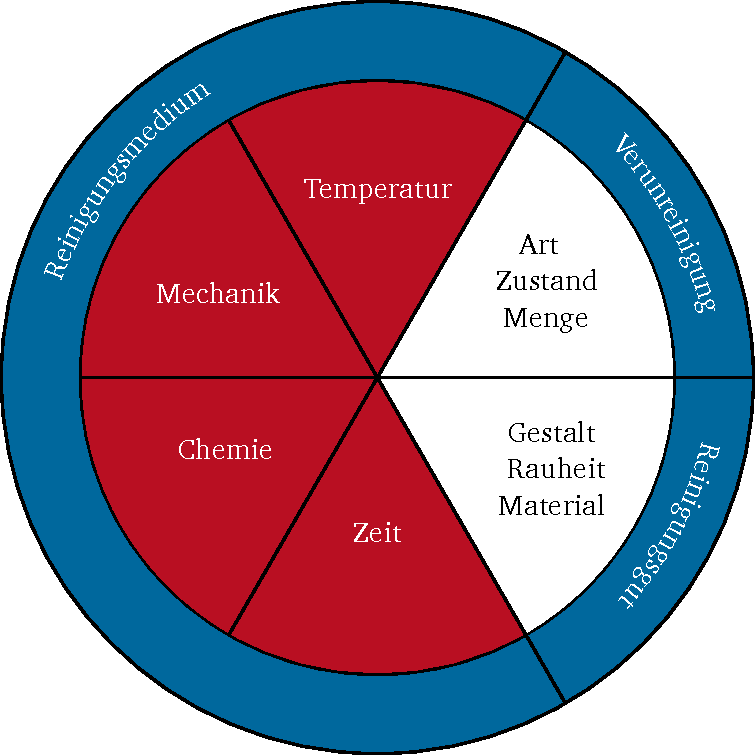
\includegraphics[width=200pt]{figures/03_Grundlagen/Erweiterter Sinnerscher Waschkreis.pdf}
 	\caption{Erweiterter Sinnerscher Waschkreis, nach [Wildbrett]}
 	\label{fig_03Erweiterter Sinnerscher Waschkreis}
 \end{figure}
 
 Seite 18 [Junge] anschauen - Zusammenfassung von Einflussfaktoren auf Energiekennzahlen verschiedener Produktionsmaschinen und Produktionsinfrastruktur - Reinigungsmaschine.
